\section{Referencia de la Estructura print\-Call}
\label{structprintCall}\index{printCall@{printCall}}
Clase de almacenamiento de una llamada a Print o a vartablasimbolos en el AST.  


{\tt \#include $<$ast.h$>$}

Diagrama de colaboraci\'{o}n para print\-Call:\begin{figure}[H]
\begin{center}
\leavevmode
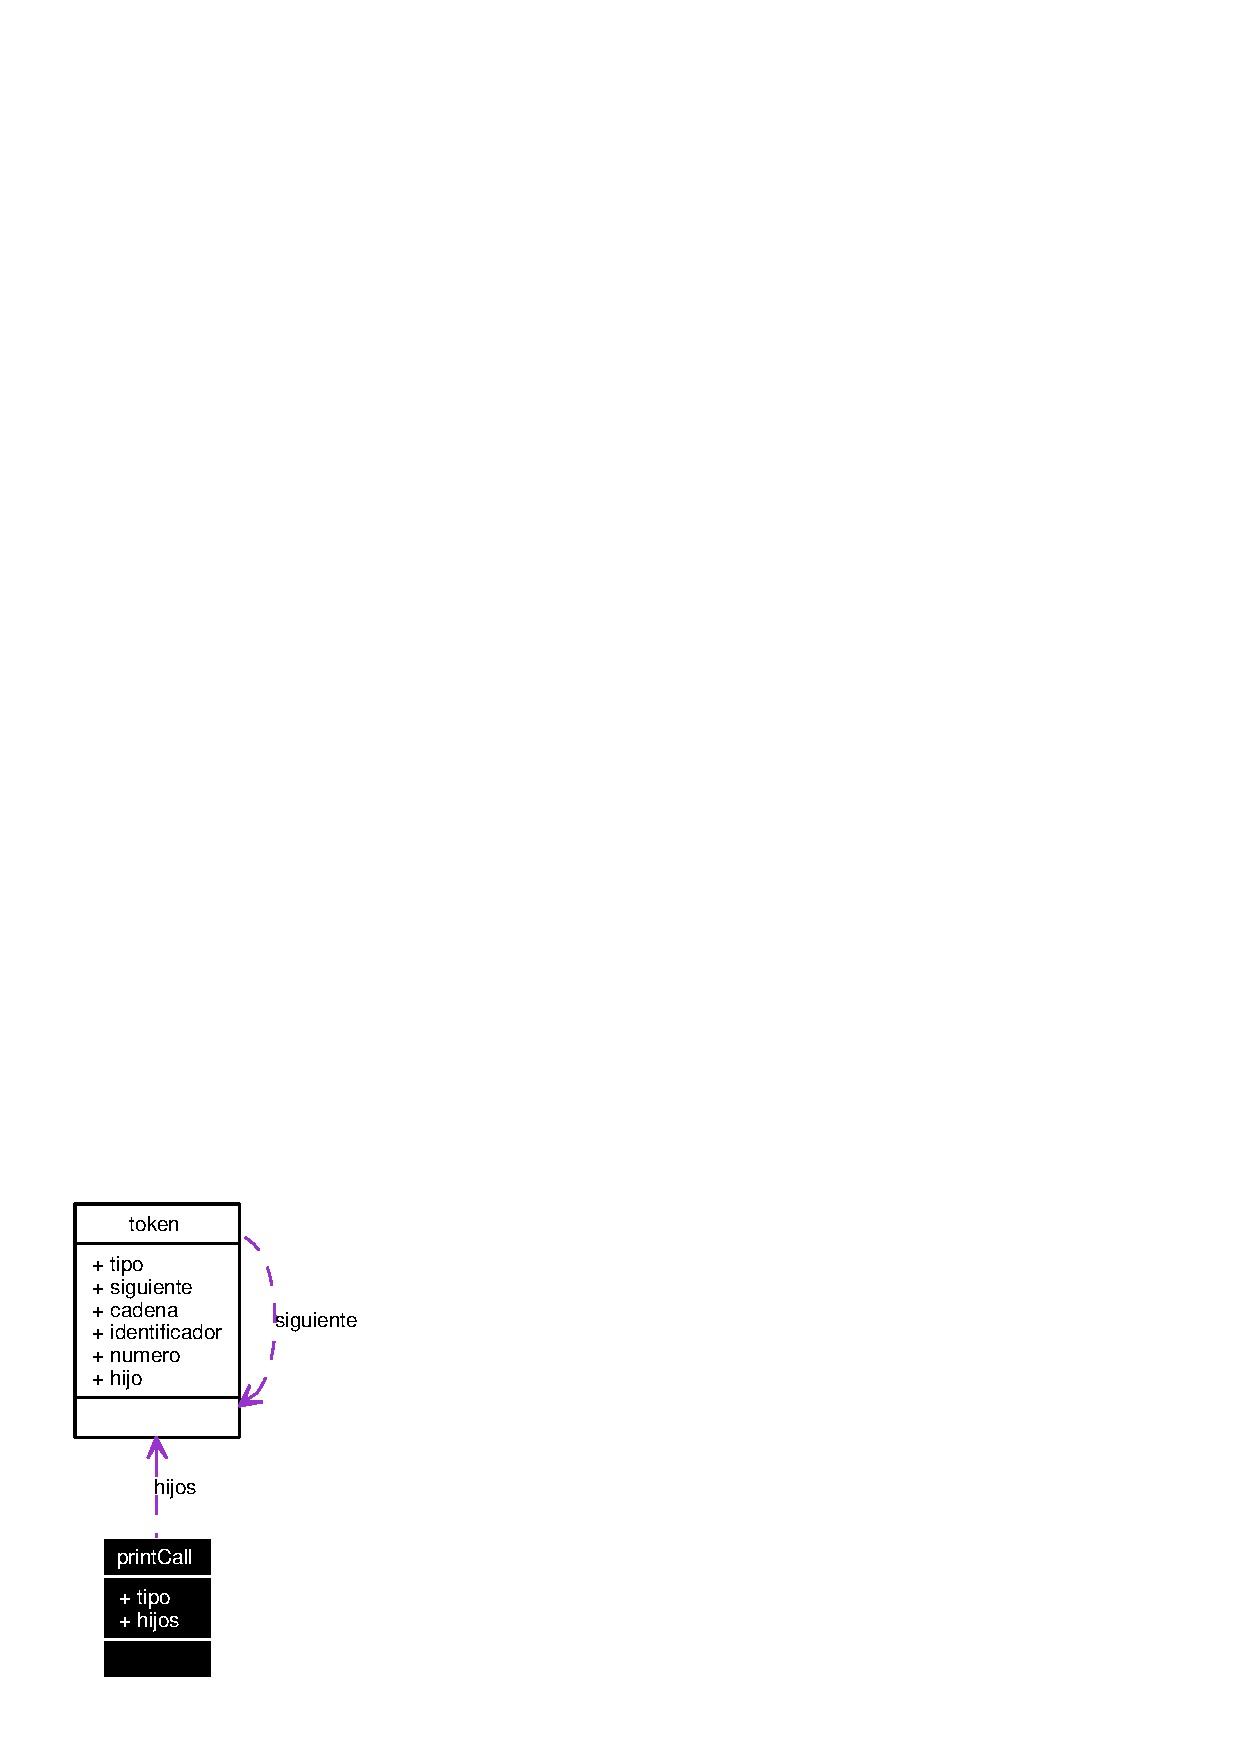
\includegraphics[width=86pt]{structprintCall__coll__graph}
\end{center}
\end{figure}
\subsection*{Atributos p\'{u}blicos}
\begin{CompactItemize}
\item 
int {\bf tipo}
\item 
{\bf token} $\ast$ {\bf hijos}
\begin{CompactList}\small\item\em Lista de tokens a imprimir. \item\end{CompactList}\end{CompactItemize}


\subsection{Descripci\'{o}n detallada}
Clase de almacenamiento de una llamada a Print o a vartablasimbolos en el AST. 



Definici\'{o}n en la l\'{\i}nea 221 del archivo ast.h.

\subsection{Documentaci\'{o}n de los datos miembro}
\index{printCall@{print\-Call}!hijos@{hijos}}
\index{hijos@{hijos}!printCall@{print\-Call}}
\subsubsection{\setlength{\rightskip}{0pt plus 5cm}{\bf token}$\ast$ {\bf print\-Call::hijos}}\label{structprintCall_o1}


Lista de tokens a imprimir. 



Definici\'{o}n en la l\'{\i}nea 223 del archivo ast.h.

Referenciado por borrar\-Print\-Call(), evaluar\-Print\-Call(), insertar\-Llamada(), y insertar\-Llamada\-Sym\-Tab().\index{printCall@{print\-Call}!tipo@{tipo}}
\index{tipo@{tipo}!printCall@{print\-Call}}
\subsubsection{\setlength{\rightskip}{0pt plus 5cm}int {\bf print\-Call::tipo}}\label{structprintCall_o0}




Definici\'{o}n en la l\'{\i}nea 222 del archivo ast.h.

Referenciado por evaluar\-Print\-Call(), insertar\-Llamada(), y insertar\-Llamada\-Sym\-Tab().

La documentaci\'{o}n para esta estructura fu\'{e} generada a partir del siguiente archivo:\begin{CompactItemize}
\item 
/media/docs/progra/c++/compiladores1/proy2/godzilla/src/{\bf ast.h}\end{CompactItemize}
